\chapter{Introduction}
\label{ch:Introduction}

This thesis implements and demonstrates a set of tools to automatically generate swarm algorithms.  \SWEEP{} (\SWEEPexpbf{}), a swarm algorithm development and simulation platform is implemented.  To demonstrate the utility of \SWEEP{}, several swarm-based algorithms are constructed for free-moving and dynamics-constrained agents, culminating in the development of basic searching and mapping algorithms for UAVs (unmanned air vehicles) tracking chemical clouds.  \ECS{} (\ECSexp{}), is implemented to evolve swarm algorithms that exhibit emergent behavior.  \ECS{} represents solutions as finite state machines, utilizes \SWEEP{} to simulate a swarm executing each state machine solution, and employs radix-based ranking to address the multi-objective nature of the problem.  As a demonstration of the ability of \ECS{}, swarm algorithms for agent dispersion, object collection, and object destruction are evolved and discussed.

\section{Motivation}

Flocking birds, foraging ants, aggregating slime molds:  these are just a few of the striking examples of self-organizing behaviors that are observed in nature.  Through a solely decentralized and reactive system, where \qw{the whole is greater than the sum of the parts,} swarms exhibit behaviors that coordinate on a global scale.  Deriving inspiration from nature, swarm theory leverages the self-organization that emerges from the interactions of multiple agents to evoke a group-level behavior that is beyond the capability of any single member of the swarm.  Swarm algorithms are most useful for problems that are amenable to an agent-based decomposition, have a dynamic nature, and do not require time-limited or optimal solutions.  

Perhaps the most advantageous aspect of swarm intelligence is the large body of work from which to draw inspiration~\cite{schechter:BoF}.  Originally, swarm theory looked to societal insects such as ants for inspiration.  For example, the method in which an ant colony will determine the closest of multiple food sources is also applicable to addressing graph-based problems such as the traveling salesman problem and the minimum spanning tree problem~\cite{bonabeau:SwarmIntelligence}.  But as more attention is focused on swarm intelligence, other sources of inspiration are identified.  Recent research is focused on extracting the implicit swarm algorithms that arise from the interactions of more intelligent organisms, \ie{} humans~\cite{palmer:HumanSwarm}.

As the size of the swarm and the complexity of the tasks increase, the opportunities for emergence increase dramatically.  In order to fully exploit the power of swarm algorithms, human programmers will need tools that extend beyond those currently available for traditional programming.  These tools will enable the programmer to work and think on a higher-level than the single agent, specifying goals and constraints for the entire swarm as opposed to loops and conditionals.  This is analogous to the development of high-level languages like C and FORTRAN that allowed programmers to focus more on concepts rather implementation.  Additionally, tools will be required for the simulation of the developed algorithm for the purposes of evaluation and testing.  Finally, tools to identify and classify emergence in a swarm will be required to optimize and verify the performance of a swarm algorithm. 

\section{Contributions}

This thesis demonstrates the use of evolutionary computing for the successful autogeneration of swarm algorithms.  In order to construct swarm algorithms, a development environment is required to facilitate experimentation and evaluation, hence the construction of a \SWEEPexp{} (\SWEEP{}).  \SWEEP{} is designed to be open and extensible.  The core \SWEEP{} architecture is constructed with minimal assumptions regarding  agent modeling, controller design, or environmental parameters.  \refFigure{SweepScreenShot} is a screenshot of \SWEEP executing a demonstration swarm algorithm.  The utility of \SWEEP{} is demonstrated through the simulation of several swarm-based scenarios including agent dispersion, task assignment, chemical cloud detection, and object manipulation.

\begin{figure}[ht]
  \centering
  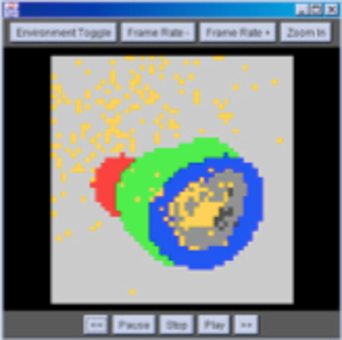
\includegraphics{SweepScreenshot}
\caption{A screenshot of \SWEEP executing a swarm algorithm}
\label{fig:SweepScreenShot}
\end{figure}

There is a small body of work related to the evolution of swarm algorithms, mostly related to the development of behaviors for swarm robotics systems.  Zaera \italic{et al.}~\cite{zaera:EvolveCollectiveBehavior} used an evolutionary method to develop behaviors for aggregation, dispersal, and schooling in fish.  Though successful in developing aggregation and dispersal algorithms, disappointing results were realized with regards to the schooling behavior, mainly due to the difficulty involved in crafting a fitness evaluation function that adequately captured the salient features of a schooling behavior.  Gaudiano, Bonabeau, and Shargel~\cite{gaudiano:EvolvingBehaviorsUAVs} used a traditional genetic algorithm to tune probabilities for  handmade probabilistic state machines used to coordinate the behaviors of a swarm of unmanned air vehicles.  Perhaps the best known example of using evolution to generate swarm behaviors is the work performed by Koza.   In Koza's work~\cite{koza:geneticprogramming-1}, he used stateless LISP S-expressions to evolve an ant-like food foraging algorithm for a small swarm of simulated ants.

This thesis extends the body of work related to the generation of swarm behaviors through evolutionary programming.  In contrast to Koza's work which used LISP S-expressions to generate state-less algorithms, this thesis represents candidate solutions as finite state machines to provide for the evolution of state-based algorithms.  The evolutionary computation system developed uses the \SWEEP{} platform to simulate candidate solutions and evaluate their fitness with respect to the multiple goals of the target scenario.  Additionally, a unique data fusion method is employed along with radix-based ranking to overcome the challenges presented by the multi-objective fitness functions required to evolve correct swarm algorithms.

\section{Summary and Outline}

This thesis focuses on the identification and implementation of tools required for the autogeneration of swarm algorithms. The work done in this thesis is organized into seven chapters.

\begin{description}
\item[\refChapter{Introduction}] lays out the focus of this thesis, the motivation for researching the autogeneration of swarm algorithms, and the contributions made by this work.
\item[\refChapter{SwarmIntelligence}] introduces the concept of swarm intelligence.  In addition, the term swarm intelligence is formally defined for this work.
\item[\refChapter{SwarmSimulationSoftware}] presents \SWEEP{} and its design.
\item[\refChapter{SweepApplications}] describes several example swarm algorithms developed with \SWEEP\ including dispersion, task assignment, and chemical cloud detection using UAVs.
\item[\refChapter{EvolutionaryGeneration}] presents \ECS, the evolutionary computing system used to evolve the swarm algorithms in \refChapter{Results}.  Here we also discuss using \SWEEP\ as a fitness function.
\item[\refChapter{Results}] explores the evolution of swarm algorithms for agent dispersion and object manipulation, a combination of object collection and object destruction.  The fitness measures used for each scenario are discussed.  In addition, evolved solutions for object manipulation are presented.
\item[\refChapter{Conclusion}] reviews the conclusions and contributions of this work, and suggests avenues for future research efforts.
\end{description}
